\documentclass[presentation,sansserif]{beamer}
\usefonttheme[onlymath]{serif}
%\renewcommand\mathfamilydefault{ppl}
%\usetheme{Warsaw}
%\usecolortheme{beetle}
\usepackage {mathpazo}
\usepackage{graphicx}
\usepackage{blindtext}

\title[Developing pop-gen models for polyploids]{Developing models for genotype uncertainty, inbreeding, and allelic inheritance in non-model polyploids}
\author[Blischak \textit{et al}.]{Paul Blischak$^1$ :: Laura Kubatko$^{1,2}$ :: Andrea Wolfe$^1$}

%\institute[OSU]{{\small Dept. of Evolution, Ecology\\ and Organismal Biology\\[0.15in] \textsc{The Ohio State University}}}

\date{}

\definecolor{itemcol}{RGB}{0,128,255}
\definecolor{back}{RGB}{1,22,39}
\definecolor{alert}{RGB}{255,0,81}
\definecolor{yell}{RGB}{255,222,0}
\setbeamercolor{alerted text}{fg=alert}
\setbeamercolor{section in toc}{fg=black, bg=black}
\setbeamercolor{item}{fg=itemcol,bg=itemcol}
\setbeamercolor{structure}{fg=itemcol!95!black}
\setbeamercolor{background canvas}{bg=white!15!black}
%\setbeamercolor{background canvas}{bg=back}
\setbeamercolor{normal text}{fg=white!95!black, bg=white!95!black}
\setbeamercolor{math text}{fg=white, bg=white}
%\setbeamertemplate{items}[square]
%\setbeamertemplate{items in toc shaded}[square]
%\setbeamertemplate{items in toc}[square]

\newcommand{\inline}[1]{\fcolorbox{white!15!black}{white!20!black}{\texttt{#1}}}

\setbeamertemplate{navigation symbols}{% 
%\insertslidenavigationsymbol 
%\insertframenavigationsymbol 
%\insertsubsectionnavigationsymbol 
%\insertsectionnavigationsymbol 
%\insertdocnavigationsymbol 
%\insertbackfindforwardnavigationsymbol \hspace{1em}%
 \usebeamerfont{footline} \insertframenumber/\inserttotalframenumber% 
 }

\begin{document}

\beamertemplatenavigationsymbolsempty

\begin{frame}[plain]
	\vspace{-1.2in}
	\titlepage
	
	\vspace{-1.2in}
	\begin{center}
	
		{\footnotesize Ohio State University 	
		\vspace{0.05in}
		
		$^1$Department of EEOB :: $^2$Department of Statistics
		}		
	\end{center}
	\vspace{-0.2in}
		
\end{frame}


\begin{frame}[t]{The world of polyploidy}

  

\end{frame}

\begin{frame}[t]{The world of polyploidy}
\framesubtitle{Types of polyploids}

	\onslide<2->{\textbf{Autopolyploids}:}
	%\pause

	\begin{center}
		\onslide<3->{\includegraphics[width=0.5\textwidth]{eps/autopolyploid-formation}}
	\end{center}
	%\pause
	
	\onslide<2->{\textbf{Allopolyploids}:}
	%\pause
	
	\begin{center}
		\onslide<4->{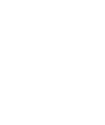
\includegraphics[width=0.5\textwidth]{eps/allopolyploid-formation}}
	\end{center}

\end{frame}

\begin{frame}[t]{Polyploid pop-gen}
  \framesubtitle{Challenges}
  
  \vspace{0.1in}
  The difficulties of making population genetic inferences in polyploids present themselves at two broad levels:
  \vspace{0.2in}
  \pause

	\begin{enumerate}
		\item \textbf{Allelic dosage}: difficult to determine the number of allele copies.
		\vspace{0.1in}
		
		\begin{itemize}
			\item Ex: Two alleles are present in a tetraploid. Is the genotype ABBB, AABB, or AAAB?
		\end{itemize}
		\vspace{0.2in}
		\pause

		\item \textbf{Allelic inheritance}: how do chromosomes pair during meiosis? Do subgenomes interact?
	\end{enumerate}
	
\end{frame}

\begin{frame}[t]{Dealing with allelic dosage}
	\pause
	\vspace{0.1in}
	Account for genotype uncertainty...
	\vspace{0.2in}

	\begin{itemize}
	\setlength\itemsep{0.2in}
		\item Our previous model used a hierarchical setup for high throughput sequencing (HTS) data, genotypes, and allele frequencies.
		\vspace{0.1in}
		\pause

		\item Joint inference on genotypes and frequencies using Gibbs sampling (implemented in the R package \textbf{polyfreqs}).
		\vspace{0.1in}
		\pause

		\item Turns out there is a better way \pause $\rightarrow$ (1) don't sample genotypes\pause, (2) don't use Gibbs sampling (too expensive).
		\vspace{0.1in}

	\end{itemize}

\end{frame}

\begin{frame}[t]{Dealing with allelic dosage}
	\framesubtitle{Genotype likelihoods}

	Instead, we pre-compute genotype likelihoods (e.g., using GATK).
	\vspace{0.2in}
	\pause
	
	$R$ -- HTS data (reads and per-base errors)
	
	$m$ -- ploidy-level
	
	$G$ -- genotype $(0,\dots,m)$
	
	$p$ -- allele frequency
	

	\pause
	\begin{equation*}
		\mathcal{L}(G) = P(R|G).
	\end{equation*}
	
	\begin{equation*}
		\mathcal{L}(p) = P(R|p) = \sum_G P(R|G)P(G|p)
	\end{equation*}
	\vspace{-0.2in}
	\pause
	
	\begin{equation*}
		= \sum_G \mathcal{L}(G)P(G|p).
	\end{equation*}

\end{frame}

\begin{frame}[t]{Assumptions}

\end{frame}

{ \setbeamercolor{background canvas}{bg=white!20!black}
\begin{frame}[c,plain]{Disequilibrium model}
	\framesubtitle{Log-likelihood surface}
	\begin{center}
		\frame{\includegraphics[width=\textwidth]{pdf/freq-phi-lik-surf2}}
	\end{center}
\end{frame}
}

{ \setbeamercolor{background canvas}{bg=white!20!black} %\setbeamercolor{math text}{fg=itemcol, bg=itemcol}
\begin{frame}[c,plain]{Allopolyploid subgenome model}
	\framesubtitle{Log-likelihood surface: $F_{st}=0.1$}
	\begin{center}
		\frame{\includegraphics[width=\textwidth]{pdf/freq1-freq2-lik-surf1}}
	\end{center}
\end{frame}
}

{ \setbeamercolor{background canvas}{bg=white!20!black} %\setbeamercolor{math text}{fg=itemcol, bg=itemcol}
\begin{frame}[c,plain]{Allopolyploid subgenome model}
	\framesubtitle{Log-likelihood surface: $F_{st}=0.5,\, \pi=0.475,\, p_1=0.962,\, p_2=0.343$}
	\begin{center}
		\frame{\includegraphics[width=\textwidth]{pdf/freqs1-freqs2-bad-lik-surf1}}
	\end{center}
\end{frame}
}

{ \setbeamercolor{background canvas}{bg=white!20!black} %\setbeamercolor{math text}{fg=itemcol, bg=itemcol}
\begin{frame}[c,plain]{Allopolyploid subgenome model}
	\framesubtitle{Log-likelihood surface: $F_{st}=0.5,\, \pi=0.922,\, p_1=0.999,\, p_2=0.414$}
	\begin{center}
		\frame{\includegraphics[width=\textwidth]{pdf/freqs1-freqs2-bad-lik-surf3}}
	\end{center}
\end{frame}
}

\subsection*{Conclusions}

\begin{frame}[t]{Conclusions}
	\fontsize{10pt}{10}\selectfont
	\begin{itemize}
		\item \textsc{Take home}: \textbf{Don't have to use genotypes as the first line of data}. Using sequencing reads is a viable solution for dealing with ADU.
		\vspace{0.2in}

		\item \textbf{The framework presented here is highly extensible}. Future work includes generalizing to both auto- and allopolyploids, more complex patterns of inheritance.
		\vspace{0.2in}

		\item \textbf{Sampling more individuals appears to be most important}. More individuals over higher sequencing coverage.
		\vspace{0.2in}

		\item \textbf{Need empirical data}. Simulations are nice, but we need to see how a model such as this works for lab-collected data.

	\end{itemize}

\end{frame}

\begin{frame}[t,plain]{Code availability}
	\fontsize{10pt}{10}\selectfont
	\begin{itemize}
		\item \textbf{polyfreqs}: an R package for the estimation of allele frequencies in autopolyploids. Available on GitHub -- \url{https://github.com/pblischak/polyfreqs}.
		\vspace{0.2in}

		\item Manuscript is currently in review, preprint is on bioR$\chi$iv -- \url{http://biorxiv.org/content/early/2015/07/02/021907}.
		\vspace{0.2in}

		\item Data and code for the simulation study and making the figures are on GitHub -- \url{https://github.com/pblischak/polyfreqs-ms-data}.
		\vspace{0.2in}

		\item Presentation slides are on fig\textbf{share}, and the \LaTeX{} source code is also on GitHub -- \url{https://github.com/pblischak/evolution2016}.
	\end{itemize}
	\vspace{0.15in}

	{\Large \alert{All these links are in the GitHub repository for this presentation: \textbf{pblischak/evolution2016}.}}

	\hfill {\tiny \#openscience}
\end{frame}

\begin{frame}[t,plain]{Acknowledgments}
  \vspace{0.2in}

  \begin{itemize}
    \setlength\itemsep{0.3in}
    \item John Novembre, Xin He, Matthew Stephens, and their lab members for the opportunity to present at U. of Chicago (and to John Blischak for organizing the visit).
    \item My labmates in the Wolfe and Kubatko labs.
    \item National Science Foundation for funding the larger project that includes the development of the models presented here.
  \end{itemize}

\end{frame}

\begin{frame}[c,plain]{}
	\begin{center}
		{\Huge Thanks!}\\
		\vspace{0.5in}
		{\LARGE Questions?}
	\end{center}
\end{frame}

\end{document}
